\question 下列( )设备可以隔离 ARP 广播帧
\par\twoch{\textcolor{red}{路由器}}{网桥}{以太网交换机}{集线器}
\begin{solution}集线器是物理层的设备,交换机和网桥都是数据链路层的设备,广播域是网络层的概念,网络层以下的设备是不可能分隔广播域的。而路由器是网络层的设备,它能够分隔广播域。
\end{solution}
\question 关于冲突域和广播域,下列说法正确的是
\par\fourch{集线器和中继器连接不同的冲突域}{网桥和二层交换机既可以隔离冲突域,也可以隔离广播域}{\textcolor{red}{路由器和三层交换机既可以隔离冲突域,也可以隔离广播域}}{通常来说,一个局域网就是一个冲突域}
\begin{solution}因为集线器和中继器无法隔离冲突域,故连接的是同一个冲突域,A选项错误;网桥和二层交换机可以划分冲突域,但不能划分广播域,B选项错误;路由器和三层交换机既可以划分冲突域,也可以划分广播域,C选项正确;D选项中要看局域网的连接设备,如果是网桥或者二层交换机连接,就不是一个冲突域。
\end{solution}
\question 一个16端口的二层以太网交换机,冲突域和广播域的个数分别是
\par\twoch{1,1}{16,16}{1,16}{\textcolor{red}{16,1}}
\begin{solution}二层以太网交换机可以隔离冲突域,由于有16个端口,所以隔开了16个冲突域,又因为二层交换机不能隔离广播域,故只有一个广播域。
\end{solution}
\question 某IP网络的连接如图3-19所示,在这种配置下IP全局广播分组不能够通过的路径是(
~)。

~
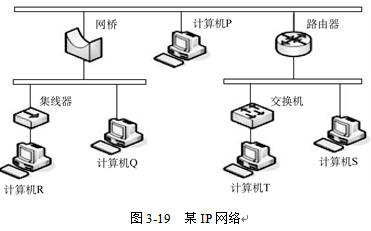
\includegraphics[width=3.33333in,height=2.08333in]{computerassets/8d1744c03d695e45dcb1f35ee5cc4189.png}
\par\fourch{计算机P和计算机Q之间的路径}{\textcolor{red}{计算机P和计算机S之间的路径}}{计算机Q和计算机R之间的路径}{计算机S和计算机T之间的路径}
\begin{solution}由于路由器可以隔离广播包的转发,所以只要是需要经过路由器的路径都是不能通过的路径。
\end{solution}
\question 在使用以太网交换机的局域网中,以下表述哪个是正确的
\par\twoch{局域网只包含一个冲突域}{\textcolor{red}{交换机的多个端口可以并行传输}}{交换机可以隔离广播域}{交换机根据LLC目的地址转发}
\begin{solution}交换机的每个端口都有它自己的冲突域,所以交换机永远不会由于冲突而丢失帧。所以A是错误的。交换机不可以隔离广播域,所以C也是错误的。LLC是逻辑链路控制,它在MAC层之上,用于向网络层提供一个接口以隐藏各种802网络之间的差异,交换机应该是按照MAC地址转发的。
\end{solution}
\question 下列网络设备中,能够抑制广播风暴的是( )。 \ding{192}.中继器 \ding{193}.集线器 \ding{194}.网桥
\ding{195}.路由器
\par\twoch{仅\ding{192}和\ding{193}}{仅\ding{194}}{仅\ding{194}和\ding{195}}{\textcolor{red}{仅\ding{195}}}
\begin{solution}一个数据帧或包被传输到本地网段上的每个结点就是广播。由于网络拓扑的设计和连接问题,或其他原因导致广播在网段内大量复制,传播数据帧,导致网络性能下降,甚至网络瘫痪,这就是广播风暴。所以要想抑制广播风暴的出现,首先这个设备应该不能随随便便地就广播。
中继器和集线器不检查数据帧的内容,仅起到放大信号、扩展网络传输规模的功效。做题的时候,考生也应该发现当集线器的一个端口收到数据后,将其从除了输入端口外的所有端口广播出去,这么随意就广播,排除。网桥对未知的目的地的数据帧总是向除了来的方向广播出去,因此无法抑制广播风暴,排除。只有路由器是严格地按照路由表的内容转发分组,不会在子网中产生大量的广播数据,因此可以有效地抑制广播风暴。
另外一种解题思路:只要可以隔离广播域就可以抑制广播风暴,显然只有路由器可以隔离广播域。
【总结】
见下表。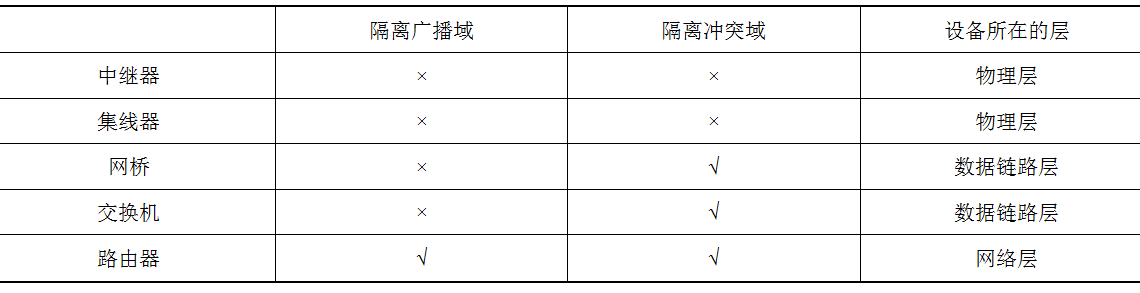
\includegraphics[width=3.46875in,height=0.89583in]{computerassets/DB7F9A377704A937E9E2FF74A32807E0.png}
\end{solution}
